6. \begin{figure}[ht!]
\center{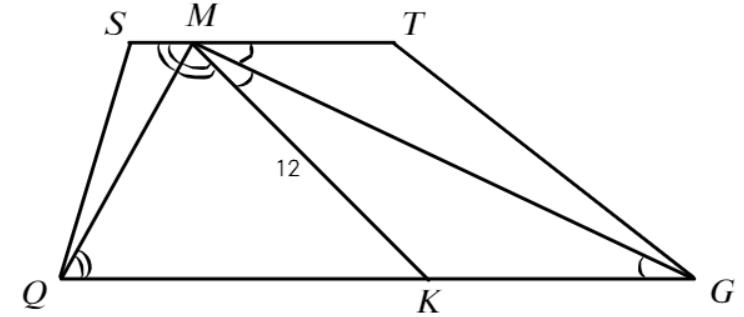
\includegraphics[scale=0.35]{g6.png}}
\end{figure}\\
Прямые $ST$ и $QG$ параллельны, а $QM$ и $MK$ --- секущие, значит $\angle SMQ = \angle MQK,$  $\angle TMG= \angle MGK$ как накрест лежащие. $MG$ и $MQ$ являются биссектрисами, поэтому $\angle SMQ = \angle QMK,$ $ \angle TMG= \angle GMK.$ Поэтому у треугольников $QMK$ и $GMK$ равны углы при основаниях, а значит они равнобедренные и $QK=MK=12,\ KG=MK=12,$ откуда $QG=QK+KG=12+12=24.$\\
